%% LyX 2.1.4 created this file.  For more info, see http://www.lyx.org/.
%% Do not edit unless you really know what you are doing.
\documentclass[10pt,english]{beamer}
\usepackage[T1]{fontenc}
\usepackage[latin9]{inputenc}
\setcounter{secnumdepth}{3}
\setcounter{tocdepth}{3}
\usepackage{babel}
\usepackage{amsmath}
\usepackage{amsthm}
\usepackage{amssymb}
\usepackage{graphicx}
\usepackage{setspace}
\setstretch{1.2}
\ifx\hypersetup\undefined
  \AtBeginDocument{%
    \hypersetup{unicode=true,pdfusetitle,
 bookmarks=true,bookmarksnumbered=false,bookmarksopen=false,
 breaklinks=false,pdfborder={0 0 0},backref=slide,colorlinks=false}
  }
\else
  \hypersetup{unicode=true,pdfusetitle,
 bookmarks=true,bookmarksnumbered=false,bookmarksopen=false,
 breaklinks=false,pdfborder={0 0 0},backref=slide,colorlinks=false}
\fi
\usepackage{breakurl}

\makeatletter
%%%%%%%%%%%%%%%%%%%%%%%%%%%%%% Textclass specific LaTeX commands.
 % this default might be overridden by plain title style
 \newcommand\makebeamertitle{\frame{\maketitle}}%
 % (ERT) argument for the TOC
 \AtBeginDocument{%
   \let\origtableofcontents=\tableofcontents
   \def\tableofcontents{\@ifnextchar[{\origtableofcontents}{\gobbletableofcontents}}
   \def\gobbletableofcontents#1{\origtableofcontents}
 }
 % plain title style, override default
 \renewcommand\makebeamertitle{\frame[plain]{\maketitle}}%
  \theoremstyle{plain}
  \newtheorem{prop}{\protect\propositionname}

%%%%%%%%%%%%%%%%%%%%%%%%%%%%%% User specified LaTeX commands.
%The next line sets the presentation design
\mode<beamer>{
\usetheme{Frankfurt} }

%The next lines determine the look of the handouts
\mode<handout> {
\setbeamertemplate{navigation symbols}{}
\usepackage{pgfpages}
\pgfpagesuselayout{2 on 1}[a4paper,border shrink=5mm] 
%\usepackage{handoutcolors}
%\setbeamercolor{title}{fg=black}
%\setbeamercolor{frametitle}{fg=black}
%\setbeamercolor{structure}{fg=black}
%\useinnertheme{circles}
}

%For handouts, simply set the "custom" parameter in the document class to "handout"

%Game theory packages
%\usepackage{sgamevar}
\usepackage{pstricks}
\usepackage{pstcol}
%\usepackage{egameps}
\usepackage{dsfont}


%\usepackage[]{beamerarticle}
%\usepackage{handoutWithNotes}
%\pgfpagesuselayout{3 on 1 with notes}[a4paper,border shrink=5mm]

%Trick to have circles everywhere in Frankfurt theme
%\usepackage{remreset}% tiny package containing just the \@removefromreset command
%\makeatletter
%\@removefromreset{subsection}{section}
%\makeatother
%\setcounter{subsection}{1}
\AtBeginSection[]{\subsection{}}

\makeatother

  \providecommand{\propositionname}{Proposition}

\begin{document}
%\AtBeginSection[]{
%\frame<beamer>{
%\frametitle{Outline}
%\tableofcontents[currentsection,currentsubsection]
%}}
%\setbeamertemplate{section in toc shaded}[default][90]
%\setbeamerfont{section in toc}{series=\bfseries}
%\setbeamerfont{section in toc shaded}{series=\normalfont}
%\beamerdefaultoverlayspecification{<+->}




\title{A Theory of Privacy}


\author{Ole Jann and Christoph Schottm�ller}


\institute{University of Copenhagen}


\date{June 7, 2016}
\makebeamertitle
\begin{frame}{Overview}


\tableofcontents{}

\end{frame}

\section{Why do we need (a theory of) privacy?}
\begin{frame}{What is Privacy?}

\begin{itemize}
\item The ability to take actions without being observed, and having interactions
with others confined to the intended recipients
\item (There are many other definitions.)
\item Privacy $\subset$ asymmetric information
\end{itemize}
\end{frame}

\begin{frame}{Privacy: A hot topic}

\begin{itemize}
\item Several Western governments systematically collect internet traffic
data, metadata, read emails, can access webcams, ...
\item People voluntarily provide lots of information on Facebook, Twitter,
...
\item Giving up information for better prices (loyalty programs, insurance
contracts)
\item Modern administrations collect lots of data and make it accessible
to many (register data!)
\item $\Rightarrow$ We need to understand what's at stake, which effects
privacy has, which trade-offs come with it
\end{itemize}
\end{frame}

\begin{frame}{Economics of Privacy: The Chicago School}

\begin{itemize}
\item The most well-known economic theory of privacy
\item Exemplified by George Stigler (1980, JLS) and Richard Posner (1981,
AER)
\item Argument:

\begin{itemize}
\item Privacy = asymmetric information
\item Asymmetric information leads to inefficiencies
\item Therefore: privacy = inefficient
\end{itemize}
\end{itemize}
\end{frame}

\begin{frame}{Popular debate: The ``Nothing to hide'' argument}

\begin{itemize}
\item ``The most common retort against privacy advocates'' (Schneier 2006)
\item Used by people at NSA, Google, ...
\item Argument:

\begin{itemize}
\item If you have nothing to hide, you have nothing to fear from giving
up your privacy
\item If you have something to hide, you should not be able to hide it!
\end{itemize}
\item (Note the similarities to the Chicago argument.)
\end{itemize}
\end{frame}

\begin{frame}{What we do}

\begin{itemize}
\item We develop an informational theory of privacy: why do people care
about it, what are the welfare effects?
\item We do not consider a ``taste for privacy'' -- instead, we derive
the individual and social benefit of privacy theoretically
\item The Chicago argument ignores two things:

\begin{itemize}
\item Information is often not perfect and unambiguous (decisions are made
by statistical discrimination; Phelps 1972, Arrow 1973)
\item People change their behavior when they know they are observed
\end{itemize}
\item It also compares with an imaginary first best (in reality, we can
never live without asymmetric information $\Rightarrow$ privacy is
about how it should be structured)
\end{itemize}
\end{frame}

\begin{frame}{4 main results + 2 extensions}

\begin{itemize}
\item Lack of privacy changes behavior systematically (``chilling effect'')
\item The chilling effect reduces overall welfare
\item Effectiveness of privacy intrusions is easily overstated
\item Privacy is redistributive -- it affects different people differently
\item Extensions:

\begin{itemize}
\item Voluntary privacy might not work
\item Lack of privacy can erode mutual trust ($\Rightarrow$ further welfare
reduction)
\end{itemize}
\end{itemize}
\end{frame}



\section{A microeconomic model}
\begin{frame}{The Model}

\begin{itemize}
\item A group of $n$ individuals have preferences over two policies, $p=0,\,1$
\item Each individual $i$ has two types: $\theta_{i}$ and $\tau_{i}$
(both are in $\mathbb{R}$)
\item $\theta_{i}$ is the policy preference (e.g. on drug legalization);
$\theta_{i}\sim\Phi(0,1)$
\item $\tau_{i}$ is the hidden type (e.g. drug use)
\item $\tau_{i}$ is correlated with $\theta_{i}$ (formally: distribution
of $\tau_{i}$ given $\theta_{i}^{'}$ F.O.S.D. the distribution of
$\tau_{i}$ given $\theta_{i}^{''}$ if $\theta_{i}^{'}>\theta_{i}^{''}$)
\item There is an opposing player (OP) who gains from treating people differently
based on $\tau_{i}$
\end{itemize}
\end{frame}

\begin{frame}{Correlation between $\theta_{i}$ and $\tau_{i}$}


\hspace*{-0.5cm}
\centering
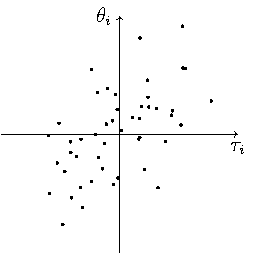
\includegraphics[scale=1.7]{graphnochilling.pdf}

\end{frame}

\begin{frame}{An example}

\begin{itemize}
\item Alice thinks drugs should be legalized and wants to write on her Facebook
profile about that
\item She is also looking for a job
\item Employers do not want to hire drug users -- but that is not observable
\item There is a correlation between stand on legalization ($\theta_{i}$)
and drug use ($\tau_{i}$)
\item Two cases: The employer can see what Alice does online, or not
\item (Acquisti and Fong 2015: Employers discriminate based on social media
profiles)
\end{itemize}
\end{frame}

\begin{frame}{Timing}

\begin{itemize}
\item Two stages:

\begin{enumerate}
\item Information aggregation: Each individual observes $\theta_{i}$ and
$\tau_{i}$, chooses $p_{i}=0$ or $p_{i}=1$. Policy $p=1$ is implemented
with probability $q(m/n)$, where $m/n$ is the proportion of individuals
that choose $p_{i}=1$
\item Interaction: An opposing player (OP) chooses, for each individual,
whether to treat them aggressively (A) or mildly (M)
\item (Payoffs are realized:)

\begin{itemize}
\item For individuals: $p\theta_{i}-\mathds{1}_{s(p_{i})=A}\delta(\tau_{i})$,
$\delta$ is an increasing function
\item For OP: $\sum_{i}\mathds{1}_{s(p_{i})=A}\tau_{i}$
\end{itemize}
\end{enumerate}
\end{itemize}
\end{frame}

\begin{frame}{What do we mean by correlation?}

\begin{itemize}
\item One attribute is \emph{predictive} of another 
\item The causality doesn't matter!
\item ``In the social sciences, everything is correlated'' (Meehl 1990)
\item Hamburger and Wallsten (2005, LA Times) about how the Republican party
targets voters:\end{itemize}
\begin{quote}
``Bourbon drinkers were more likely to be Republican, while gin was
a Democrat\textquoteright s drink. ... Democrats preferred Volvos;
Ford and Chevy owners were most likely Republicans. People with call-waiting
service on their telephones were predominantly Republican.\textquotedblright{}
\end{quote}
\end{frame}

\begin{frame}{Correlation and Machine Learning}


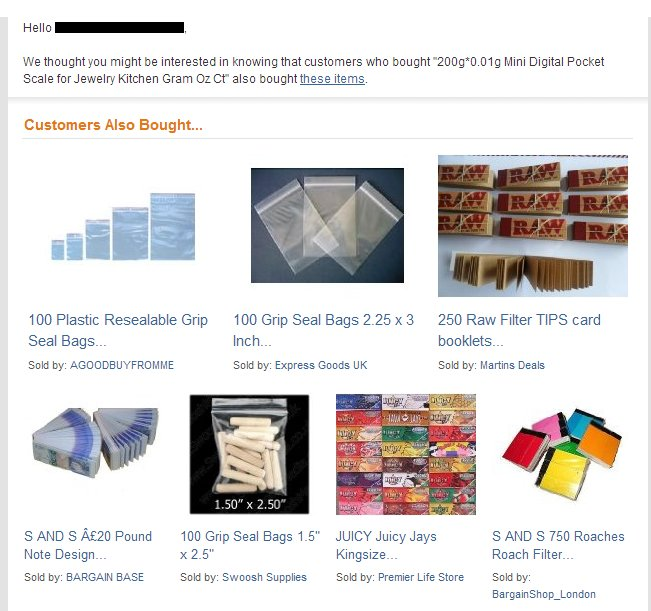
\includegraphics[scale=0.4]{example1}

\end{frame}

\begin{frame}{How we solve the game}

\begin{itemize}
\item We consider two cases: 

\begin{itemize}
\item Privacy: OP can not observe $p_{i}$, has to treat everybody the same
(we assume: mild, $M$)
\item No Privacy: OP can observe $p_{i}$ before choosing how to treat a
person
\end{itemize}
\item We show that individuals use cutoff strategies ($p=1$ if $\theta_{i}>t(\tau_{i})$)
\item We consider cutoffs and OP choices under the two cases
\end{itemize}
\end{frame}

\section{Four Results}
\begin{frame}{R1: The chilling effect}

\begin{prop}
For all $i$, the equilibrium cutoff $t(\tau_{i})$ is higher without
privacy. The difference $t^{\mathrm{no\,privacy}}(\tau_{i})-t^{\mathrm{privacy}}(\tau_{i})$
is increasing in $\tau_{i}$.\end{prop}
\begin{itemize}
\item People with positive, but small $\theta_{i}$ choose $p_{i}=0$ instead
of 1
\item OP still plays $M$ against $p_{i}=0$, but $A$ with positive probability
against $p_{i}=1$
\end{itemize}
\end{frame}

\begin{frame}{Chilling effect: Graph}


\hspace*{-0.5cm}
\centering
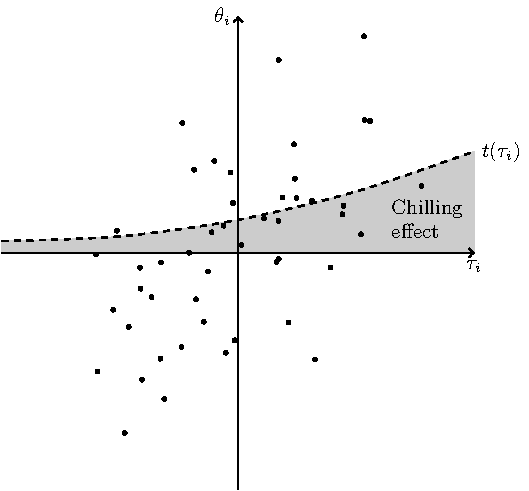
\includegraphics[scale=0.95]{graphchilling.pdf}

\end{frame}

\begin{frame}{R2: The chilling effect reduces welfare}

\begin{prop}
1) If OP uses a mixed strategy in the no-privacy equilibrium, then
privacy welfare-dominates no privacy

2) If OP uses a pure strategy in the no-privacy equilibrium, then
privacy welfare-dominates no privacy for large $n$. (+ technical
assumptions)\end{prop}
\begin{itemize}
\item $\Rightarrow$ The chilling effect impairs information aggregation
and reduces welfare
\item (We consider welfare separately for the individuals and OP.)
\end{itemize}
\end{frame}

\begin{frame}{Alice and the Chilling Effect}

\begin{itemize}
\item Alice knows that she lowers her chances of being employed if she posts
her opinion about drug legalization
\item Therefore she doesn't (or misrepresents her views) $\Rightarrow$
chilling effect
\item People who oppose legalization have no such problem
\item The public debate is systematically skewed
\item $\Rightarrow$ the welfare-optimal policy is less likely to be implemented,
which lowers expected welfare
\end{itemize}
\end{frame}

\begin{frame}{R3: Surveillance performs worse than expected$^{*}$}

\begin{itemize}
\item Naively, one could expect that taking away privacy (through surveillance,
buying data, starting to use data that is already available) delivers
large surplusses to the OP
\item But the chilling effect reduces the correlation between $p_{i}$ and
$\tau_{i}$
\item Formally, we can show:\end{itemize}
\begin{prop}
OP's payoff without privacy is lower if citizens use the cutoffs $t^{\mathrm{no\,privacy}}(\tau_{i})$
than if they use $t^{\mathrm{privacy}}(\tau_{i})$.
\end{prop}
\end{frame}

\begin{frame}{R4: Privacy has different influences on different people}

\begin{itemize}
\item Note that people with $\theta_{i}<0$ are better off \emph{without}
privacy, since that makes it more likely that their preferred policy
is implemented (and they always get treated mildly)
\item People who are subject to the chilling effect are worse off
\item People with $\theta_{i}>t^{\mathrm{no\,privacy}}(\tau_{i})$ are worst
off: they lose $\delta(\tau_{i})$ \emph{and} their preferred option
is less likely
\item $\Rightarrow$ privacy is redistributive
\end{itemize}
\end{frame}

\begin{frame}{Extension: Voluntary privacy}

\begin{itemize}
\item Assume that individuals can choose whether OP can observe their $p_{i}$
or not
\item There are several equilibria: 

\begin{enumerate}
\item Everybody chooses privacy, OP plays $M$
\item Only people with $p_{i}=1$ choose privacy, or nobody chooses privacy
$\Rightarrow$ as before
\item (Some intermediary equilibria)
\end{enumerate}
\item 1 is not stable under the D1 criterium (Banks and Sobel 1987)
\item $\Rightarrow$ Privacy might not work if it is voluntary, it has to
be imposed
\item <2->(Similar to Schelling's (1960) argument about the secret ballot.)
\end{itemize}
\end{frame}

\begin{frame}{Extension: Defensive actions}

\begin{itemize}
\item Assume that each person can take a costly defensive action to lower
the disutility of being treated aggressively by OP at the same time
as choosing $p_{i}$
\item This action also lowers the utility of OP
\item Without privacy, a person choosing $p_{i}=1$ also chooses the defensive
action
\item In our example: Alice could hire a lawyer if she supports legalization
\item Everybody is worse off
\item $\Rightarrow$ Lack of privacy can lead to a ``spiral of distrust'',
further decreases welfare
\end{itemize}
\end{frame}

\section{Examples}
\begin{frame}{Credit scoring}

\begin{itemize}
\item A bank has to decide to whom to lend; repayment probability ($\tau_{i}$)
is not directly observable
\item Consider two preferences (two different $\theta_{i}$) that are predictive
of $\tau_{i}$: Taste for education ($\Rightarrow$ education level)
and taste in music
\item Low education and a preference for rap music predict low repayment
probability
\item (There are ``social scoring'' companies who collect data like that,
Facebook has a patent on a method)
\item <2->There is a chilling effect in both cases, but in the first we
might consider it desirable!?
\item <3->Should the bank be allowed to use data on music taste? (``Equal
Credit Opportunity Act'' outlaws ``redlining'' in the US)
\end{itemize}



\end{frame}

\begin{frame}{Work in committees}

\begin{itemize}
\item A committee is debating two policies (e.g. raise interest rates or
not)
\item The debate and vote can either be in secret or in public
\item There is a correlation between policy preference $\theta_{i}$ and
competence $\tau_{i}$
\item Members worry about being perceived as incompetent; advocate less
radical positions
\item <2->The Fed is forced to publish minutes of FOMC meetings since 1993;
studies show an increase in conformity and a decrease of disagreement
with the chairman (Meade and Stasavage 2008)
\item <2->Thomas Hoenig, President of the Kansas City Fed: ``The tape
has had some chilling effect on our discussions. I see a lot more
people reading their statements.''
\end{itemize}
\end{frame}

\begin{frame}{Conclusion}

\begin{itemize}
\item Privacy is a thorny issue with many facets
\item We propose a simple model to understand what privacy is, why it is
important for welfare \emph{from an informational perspective}
\item Our model crystallizes some policy questions:

\begin{itemize}
\item Which data should be available, usable about people?
\item Is it enough to give them the option of privacy?
\item How open should government be?
\item If privacy is redistributive -- should that influence how much privacy
people get?
\item <2->Note: freedom of expression is also redistributive. Friedman
(1972) argues that it should still be universal
\end{itemize}
\end{itemize}



\end{frame}

\end{document}
